\chapter{A Quick (and Hopefully Painless) Ride Through Ruby (with Cartoon Foxes)}
\begin{figure}[h]
  \centering
  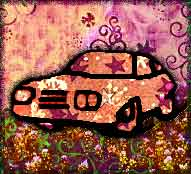
\includegraphics[width=0.2\textwidth]{image/why/chapter-3.jpg}
\end{figure}

\begin{figure}[h]
  \centering
  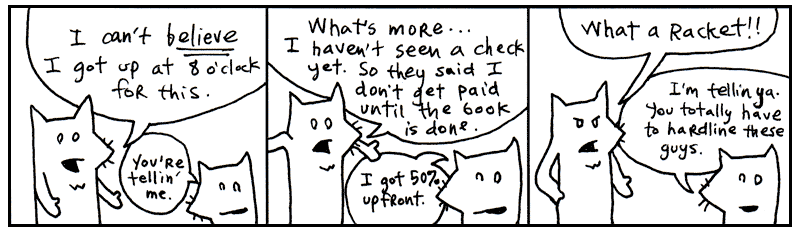
\includegraphics[width=0.75\textwidth]{image/why/foxes-1.png}
  \caption{出现了, 小狐狸们}
\end{figure}

哈, 没错, 就是这两小只. 糟了, 我的哮喘又发作了, 
所以我现在要去拿我的气雾剂了, 一会见. 

\begin{figure}[h]
  \centering
  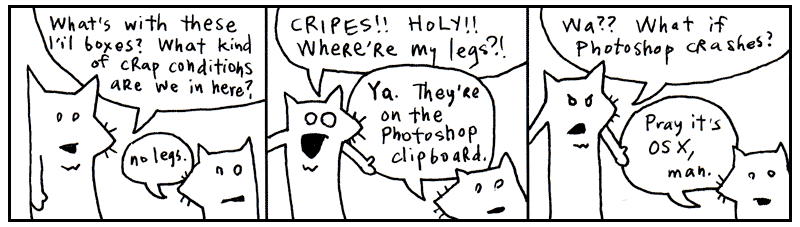
\includegraphics[width=0.75\textwidth]{image/why/foxes-2.png}
  \caption{foxes in boxes}
\end{figure}

这章的故事里面有很多的故事没准会让你潸然泪下. 
\footnote{原句我猜测应该是利用了双关: I'm told that this chapter is best accompanied by a \textbf{rag}. Something you can mop your face with as the sweat pours off your face. 其中 rag 有恶作剧和抹布的两种意思. 但是根据书的标题, 感觉这样翻译比较好一点. 这里借鉴了\href{http://codecly259.github.io/poignant-guide-cn/book/chapter-3.html}{中文的翻译版本}}

别废话了, 我们现在就快速地看看 Ruby 的大致的特性吧. 
就好像是高速吟唱ABC字母歌一样. 
\footnote{原句是: Like striking every match in a box as quickly as can be done. (就像是尽可能快地划亮火柴盒里面的所有火柴一样. )我认为不够能够表达接下来的内容. }

\section{语言以及我所指的语言}
\begin{figure}[h]
  \centering
  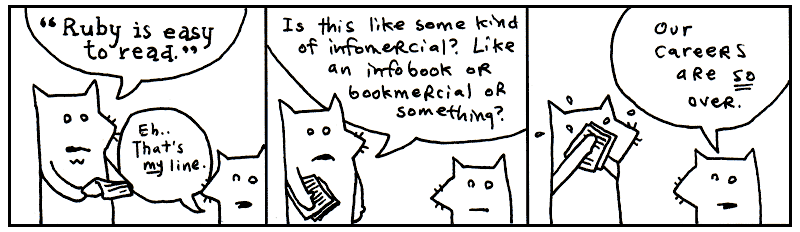
\includegraphics[width=0.75\textwidth]{image/why/foxes-3.png}
  \caption{我们这两只狐狸朋友终于明白了他们一无是处的窘境了}
\end{figure}

我的良心不允许我将 Ruby 叫做一种\emph{计算机} 语言. 
这样的话就听起来像是 Ruby 原来只是用于计算机专业的用途, 
并且从头到尾就只是设计出来为了对电脑指手画脚发送指令的, 让我们这些 
coders 看起来不过就是些在计算机领地里面要求公民身份的外国人一样. 
这样的话, 我们岂不就只是个会计算机语言翻译机器了吗? 

但是如果你的大脑都开始使用一个语言进行思考, 
你开始使用这个语言中的词汇和口语来表达你的思想, 
你还会叫这个语言仅仅是计算机语言吗? 想想看吧, 计算机可不会做这样的事.
所以你又怎么能够将 Ruby 叫做是计算机语言呢? 
它就是我们自然表达的语言啊. 

我们可不能再说 Ruby 只是 \emph{计算机} 语言了. 
它是\emph{coderspeak}, 是我们的思维的语言. \\

\textbf{试试看将下面的代码读出来: }
\begin{quotation}
  \begin{minted}{ruby}
    5.times { print "Odelay!" }
  \end{minted}
\end{quotation}

在中文里面\footnote{原文是"英语"}, 句号, 叹号和括号一样的标点符号是无声的, 
它们会给单词赋予意义, 帮助读者们在字里行间理解作者想要传递的意义. 
所以我们来试试读出上面的代码: \emph{五次打印出"Odelay!"}
\footnote{Five times print "Odelay!" 或者调换一下顺序, 打印五次"Odelay!"}

没错, 你读出的就正好就是这段小小的 Ruby 代码所做的事情. 
Beck的\href{http://whiskeyclone.net/ghost/songinfo.php?songID=175}{mutated Spanish}里的呼吼也将在他的电脑屏幕里面打印五次. 
\footnote{人类的本质就是复读机}

\textbf{试试看将下面的代码读出来: }
\begin{quotation}
  \begin{minted}{ruby}
    exit unless "restaurant".include? "aura"
  \end{minted}
\end{quotation}

在这个问题里面, 我们做了一点点十分基础的检查(reality check). 
我们的程序将会\textbf{exit}(也就是结束运行并退出)\textbf{unless}(除非)
我们的单词\textbf{restaurant}(餐厅)里面包含(也就是\textbf{includes})
单词\textbf{aura}. 这一次用中文来说就是: 退出, 
除非餐厅(restaurant)里面有气氛(aura). 
\footnote{又是一个双关. }

你可曾见过像这样方便地使用问号的编程语言呢? 
Ruby 使用像感叹号和问号之类的标点符号来增加代码的可读性. 
既然我们在上面写的是一个问句, 那为何不让它变得更加清晰易读呢? 

\textbf{试试看将下面的代码读出来: }
\begin{quotation}
  \begin{minted}{ruby}
    ['toast', 'cheese', 'wine'].each { |food| print food.capitalize  }
  \end{minted}
\end{quotation}

尽管这个看起来不是有点难读, 并且和前面的例子相比, 它不是很像一个句子. 
但是我还是会鼓励你将它读出来. 因为 Ruby 代码有时候可能读以来像是英语, 
它有时候也会读起来像是被缩写了的英语, 所以你只要把它稍微转换一下, 
就可以这样子: \emph{With the words 'toast', 'cheese', and 'wine': take each food and print it capitalized.}
(我有一堆单词(食物)'toast', 'cheese'和'wine', 分别从里面拿出每一个食物, 
然后将它用大写的形式输出到屏幕上. )

然后计算机将会彬彬有礼地输出\underline{Toast}, \underline{Cheese}
以及\underline{Wine}.

在这个时候, 你也许会好奇这些符号到底是如何相互之间联系在一起的. 
估计你现在正在为这些点号和括号到底是干什么用的而烦恼. 
\footnote{原文: Smotchkkiss is wondering what the dots and brackets mean. 不清楚这个是什么意思}
别担心, 我将在下一节进行一个介绍. 

现在你只要知道 Ruby 基本上是由一个个语句组成的. 虽然严格意义上来说, 
这些语句并不是语法正确的英文句子, 
它们更像是一堆组合在一起来传递特定的想法的单词和标点符号. 
这些语句可以形成一本书, 一篇文章甚至如果他们组织得当, 能够形成一整部小说, 
一部不仅能被人能阅读的小说, 也同时能够被计算机所理解. 

\section{语句的组成部分}
就像是臭鼬身上的白色条纹和新娘子的白色婚纱一样富有标志性, 
\footnote{原文就是这样, Just like the white stripe down a skunk's back and the winding, white train of a bride, why先生的比喻十分的有趣, 经过翻译感觉就像是吃麻辣烫前先将佐料过一遍白开水, 原本的味道全没了. }
许多 Ruby 的语句在形式上就有很多的标志(visual cues)来帮助你来辨认他们. 
比如标点和大写可以让你的大脑在看到这一堆代码的一瞬间就认出它们, 
就好像是你的潜意识在大喊: \emph{嘿, 我认识这个家伙! }
于是你就能够轻松区分(name-drop)这些组成部分并且融入 Rubyists 的交流之中. 

接下去我会在形式上给出 Ruby 里面的不同的语句组成部分的介绍, 
现在我不会细致地去解释里面的细节(这些会在这本书的其他部分介绍), 
并且你也不必费劲去理解这些解释和定义. 你只需要能够在这章结束的时候, 
能够在一个 Ruby 程序中认出这些部分就可以了. 
\footnote{这段有点不太好翻译: Try to focus on the look of each of these parts of speech. The rest of the book will detail the specifics. I give short descriptions for each part of speech, but you don't have to understand the explanation. By the end of this chapter, you should be able to recognize every part of a Ruby program.}

好的, 让我们来关注下面的这些语素吧: 
\footnote{在这里我用了语素这个该死的语法名称, 只是因为我词汇缺乏而已, 请见谅. 并且在下面的翻译中, 我不会将英文的叫法给翻译了, 因为这个我觉得是一种专有名词, 翻译了总觉得有点怪怪的. }

\subsection*{Variables}
任何简单的小写单词在 Ruby 里面就是一种 variable(变量). 
Variable 可以由字母, 数字和下划线组成. 

\begin{quotation}
  \mintinline{ruby}{x}, \mintinline{ruby}{y}, \mintinline{ruby}{banana2}
  或者是 \mintinline{ruby}{phone_a_quail} 就是一些例子
\end{quotation}

Variable 就像是绰号. 还记得曾经所有人都叫你臭彼得(Stinky Pete)的时候吗?
只要你一出现, 总会有人大喊: "嘿, 滚出去, 臭彼得! " 
然后所有人都奇迹般地知道了"臭彼得"就是你. 
\footnote{呃, 虽然我也有绰号, 但是却是一个有意思的绰号. 不知道why经历了一个怎么样的学校生活, 这个故事太惨了. 后面的例子我就不一一吐槽了, 但是我真的应该是没有乱翻译. 就是, 这些故事有点悲惨. }

使用 variable, 你就像是给自己经常使用的东西取了一个绰号. 举个例子. 
假如说你开了一个孤儿院. 这是一个十分抠门的孤儿院. 当 Warbucks 老爹
(Daddy Warbucks) 来领养孩子的时候, 我们还强迫他再从我们这里买一个
\textbf{一百二十一点零八美分}的泰迪熊 -- 因为它们是这些孩子们
在这噩梦般的孤儿院里面的唯一的精神慰藉了. 

\begin{minted}{ruby}
  teddy_bear_fee = 121.08
\end{minted}

然后, 当你要着铃铛叫他前去收银台(那里有一台运行着 Ruby 
的性能强大的收银机)去结账, 然后你要将他的所有的开销都加在一起, 
记作\textbf{total}. 

\begin{minted}{ruby}
  total = orphan_fee + teddy_bear_fee + gratuity
\end{minted}

这些变量的绰号实在是帮大忙了. 
\footnote{上面的公式, 假如把里面的英文翻译一下的话就是: 总计 = 孤儿的领养费用 + 泰迪熊的价格 + 小费, 是不是非常好理解, 比起$121.08$这样不明所以的数字起来, 简直就是小学问题了. }
并且我确信, 在这肮脏的地下儿童交易里面, 任何的小聪明都是值得一试的. 

\begin{figure}[h]
  \centering
  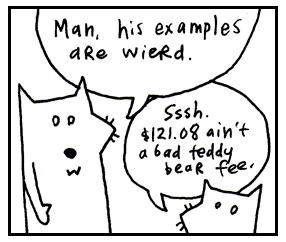
\includegraphics[width=0.25\textwidth]{image/why/foxes-4a.png}
  \caption{这帮家伙嘲笑我的例子}
\end{figure}

\subsection*{Numbers}
最常见的一种数的类型是\emph{integer}, 
它们是带着\textbf{正号或负号}的\textbf{一系列的数字}. 

\begin{quotation}
  \mintinline{ruby}{1}, \mintinline{ruby}{23}, 以及\mintinline{ruby}{-10000}就是一些例子
\end{quotation}

虽然数字里面不能出现逗号, 但是却可以出现下划线. 
所以假如你想要将数字每三位进行分割来增加可读性的话, 可以使用下划线. 

\begin{quotation}
  \begin{minted}{ruby}
    population = 12_000_000_000
  \end{minted}
\end{quotation}

在 Ruby 里面, 小数(decimal numbers)被称为\emph{floats}(浮点数). 
Floats 类型的(也就是小数)有两种形式: \textbf{带小数点的}
或者是\textbf{用科学记数法来表示的}. 

\begin{quotation}
  \mintinline{ruby}{3.14}, \mintinline{ruby}{-808.08}以及\mintinline{ruby}{12.043e-04}就是一些例子. 
\end{quotation}

\subsection*{Strings}
Stings(字符串)是一堆被\textbf{引号}包围的任意字符
(字母啊, 数字啊, 标点符号啊都行). 
无论是单引号还是双引号都能够用来形成Strings. 

\begin{quotation}
  \mintinline{ruby}{"sealab"}, \mintinline{ruby}{'2021'}, 或者是\mintinline{ruby}{"These cartoons are hilarious!"} 就是一些例子. 
\end{quotation}

当你将这些符号字母用引号包在一起之后, 它们就被储存在一个string里面. 

想象一下这个场景: 一堆名流的晚宴上, 熙熙攘攘的谈话声混在一起, 
场面十分的聒噪. 你是一个记者, 想要从这堆噪音中捕捉到名流的话语. 
"我比你们更加精明, " Avril Lavigne 说到, "并且我知道经商的秘诀
-- 就是你该做些什么以及怎么做到它. "
\footnote{原文是英文, 并且我对代码里面的英文保留了, 代码里面的英文可以参考这里的翻译. }

\begin{quotation}
  \begin{minted}{ruby}
    avril_quote = "I'm a lot wiser.  Now I know
    what the business is like -- what you have
    to do and how to work it."
  \end{minted}
\end{quotation}

就像我们之前把一个数储存在\textbf{teddy\_bear\_fee} variable里面一样, 
现在我们把一组字符(也就是一段string)储存在了\textbf{avril\_quote} 
variable里面. 然后你这个记者把这段名言发送给了印刷人员. 
这位印刷人员恰好使用的是 Ruby 来进行他们的印刷工作: 

\begin{quotation}
  \begin{minted}{ruby}
    print oprah_quote
    print avril_quote
    print ashlee_simpson_debacle  
  \end{minted}
\end{quotation}

\begin{figure}[h]
  \centering
  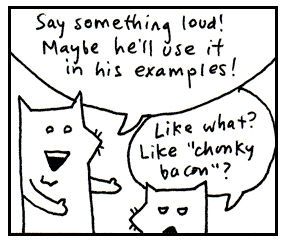
\includegraphics[width=0.25\textwidth]{image/why/foxes-4b.png}
  \caption{他们想要帮我想例子}
\end{figure}

\subsection*{Symbols}
Symbols(符号)看起来就像是变量一样. 它们都包含字母, 数字, 还有下划线. 
但是symbols\textbf{是以一个冒号开头的}. 

\begin{quotation}
  \mintinline{ruby}{:a}, \mintinline{ruby}{:b}, 或者\mintinline{ruby}{:ponce_de_leon}就是一些例子. 
\end{quotation}

Symbols 相较于strings更加的轻便. 假如你想要使用像string一样的标记, 
但是又不想将它们用来打印的话, 使用symbol会比较方便. 

或者你可以理解为symbol对于电脑来说更加容易处理. 
symbol前面的冒号就像是插在椰果上的吸管, 让计算机能够轻松地吸取处理它, 
啊, 真是甜蜜而又轻松啊. 
\footnote{原文是: It's like an antacid. The colon indicates the bubbles trickling up from your computer's stomach as it digests the symbol. Ah. Sweet, sweet relief. 大意就是说symbol对于计算机来说比较容易处理, 为了保留原来的比较有趣的比喻, 所以我换了一个比喻. 因为翻译不过来. \\这里追加一个解释, 因为在计算机里面, 符号和字符串还是有一点点不一样的, 对于字符串, 计算机是对每一个字符进行一个比较后才能说两个字符串是一样的, 而对于符号, 计算机内部是将其转换为一个特殊的数字, 这个数字比较方便比较, 储存和比较的效率比较高. }

\begin{figure}[h]
  \centering
  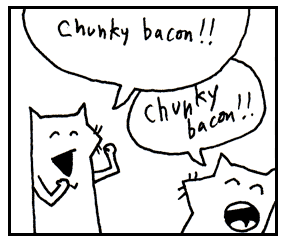
\includegraphics[width=0.25\textwidth]{image/why/foxes-4c.png}
  \caption{Chunky bacon!!(烟熏肉! )}
\end{figure}

\subsection*{Constants}
Constants(常量)有点像是variables, 
但是constant是\textbf{用大写字母开头的}. 
假如variables像是Ruby里面的名词(nouns), 那么constants就像是专有名词(proper nouns). 

\begin{quotation}
  \mintinline{ruby}{Time}, \mintinline{ruby}{Array}, 或者\mintinline{ruby}{Bunny_Lake_is_Missing}就是一些例子. 
\end{quotation}

在英语中, 专有名词都是大写字母开头的. 就像是帝国大厦(Empire State Building)一般. 你不能够移动帝国大厦. 你也不能定义它为什么其他的东西. 
\footnote{假如为了地方特色化的话, 可以变成人民大会堂或者是天安门广场一样的东西. }
专有名词大概就是像那样的东西. 它们表示的是一些比较特别的东西, 
一般人们不想要它随便地变化. 

同样的, constant也不应该在被他们声明了之后被改变. 

\begin{quotation}
  \begin{minted}{ruby}
    EmpireStateBuilding = "350 5th Avenue, NYC, NY"
  \end{minted}
\end{quotation}

假如我们尝试去修改这个constant, Ruby会皱着眉毛抱怨我们. 
\footnote{实际上还是可以改的, 毕竟Ruby很随意. 假如是别的严格的语言, 就会像是去星巴克点小杯一样的坑爹故事一样了. 因为你不合规矩, 所以就会被骂了. 但是Ruby就像是个宽容的同辈的朋友, 会容忍你的任性. }

\begin{figure}[h]
  \centering
  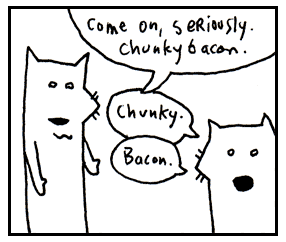
\includegraphics[width=0.25\textwidth]{image/why/foxes-4d.png}
  \caption{上啊, chunky bacon}
\end{figure}

\subsection*{Methods}
假如varibles和constants像是名词, 那么methods就像是动词(verbs). 
Methods通常跟在variable或constant的后面, 用一个\textbf{点号}来分割. 
你应该在生活中早就见过类似的东西了: 
\footnote{原文: Methods are usually attached to the end of variables and constants by a dot. You've already seen methods at work. 嗯, 翻译的感觉差不多. }

\begin{quotation}
  \begin{minted}{ruby}
    front_door.open
  \end{minted}
\end{quotation}

在上面的例子里面, method是\textbf{open}. 在上面的那一行语句里面, 
它就像是一个动词, 一个操作. 在某些情况下, 你能够看到多个动词
串联在一起使用. 

\begin{quotation}
  \begin{minted}{ruby}
    front_door.open.close
  \end{minted}
\end{quotation}

上面的语句里面, 我们控制计算机把前门(front door)打开了又立刻关上了. 

\begin{quotation}
  \begin{minted}{ruby}
    front_door.is_open?
  \end{minted}
\end{quotation}

上面的语句也同样是一个操作(action). 我们控制计算机去检查门(front door)
有没有打开. 本来这个method应该叫做
\mintinline{ruby}{Door.test_to_see_if_its_open}, 
但是\mintinline{ruby}{is_open?}这个名字更加的简洁和适当. 
在 Ruby 里面, 感叹号和问号都可以被用于method名字里面. 
\footnote{有助于让method的名字更加好懂. }

\subsection*{Method arguments}
一个method(方法)可能需要一些信息输入(method argument)才能够执行它的操作. 
比如说, 假如我们想要让计算机给我们的门涂上一层油漆, 
我们就需要告诉它该用什么颜色的油漆. 
\footnote{不让你也不想计算机随便给你的门涂上奇怪的颜色吧. }

\begin{quotation}
  \begin{minted}{ruby}
    front_door.paint( 3, :red )
  \end{minted}
\end{quotation}

上面的语句将前门(front door)上了三重红色的漆. 

想象一下, 在method的背后有一个神奇的机械和隐秘的管道
(将我们的参数传递给method, 或者说计算机来执行). 
我们的圆括号就是那个圆圆的, 湿漉漉的管道内壁; 
我们的逗号就像是每一个参数(argument)长的脚, 这些脚贴在管道上, 
因为最后一个参数将它的脚悄悄地藏了起来, 所以你看不见它们. 
\footnote{这一段比较难翻译, 原文是: Think of it as an inner tube the method is pulling along, containing its extra instructions. The parentheses form the wet, round edges of the inner tube. The commas are the feet of each argument, sticking over the edge. The last argument has its feet tucked under so they don't show. 大意就是method的参数之间用逗号相互隔开, 通过括号传递给method. }

就像是一台机器里面有许多的管道一样, methods和参数也是可以被串在一起使用的. \footnote{Like a boat pulling many inner tubes, methods with arguments can be chained.}

\begin{quotation}
  \begin{minted}{ruby}
    front_door.paint( 3, :red ).dry( 30 ).close()
  \end{minted}
\end{quotation}

上面的例子里面我们为门涂了三层红漆, 然后干燥了30分钟, 然后关上了门. 
尽管最后一个method没有任何的参数, 如果你喜欢的话也可以在后面加上括号. 
虽然一般来说, 在机器里面放一条空管道是挺没用的, 所以这对括号常被忽略. 

还有一些methods(比如\mintinline{ruby}{print})属于kernel methods
(kernel内核). 这些方法可以在 Ruby 的各个区域被调用. 真是因为它们很普遍
(common), 所以你不必加上点号. 

\begin{quotation}
  \begin{minted}{ruby}
    print "See, no dot."
  \end{minted}
\end{quotation}

\subsection*{Class methods}
正如上面介绍的methods一样(上面的methods也叫做\textbf{instance} 
methods), 而class methods(类方法)虽然也跟在variable和constant后面, 
但是并不是使用点号分隔, 而是\textbf{两个冒号}. 

\begin{quotation}
  \begin{minted}{ruby}
    Door::new( :oak )
  \end{minted}
\end{quotation}

正如上面的例子展示的一样, 一个\mintinline{ruby}{new} class method
(叫做\textbf{new}的类方法)是用来创造一些东西的. 在上面的例子里面, 
我们请求 Ruby 为我们制作一个新的oak(橡树)门. 
\footnote{其实写成\mintinline{ruby}{Door.new}也是可以创建一个新的实例对象了, 这里就有点让人难懂了, 不过应该不是什么大问题. }
当然, Ruby 需要知道如何去做一扇门 -- 肯定要有一堆木料, 一堆伐木工人, 
以及那些双人锯. 

\begin{figure}[h]
  \centering
  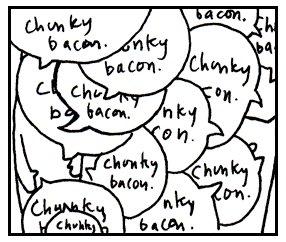
\includegraphics[width=0.25\textwidth]{image/why/foxes-4e.png}
  \caption{可真是一堆的chunky bacon呢}
\end{figure}

\subsection*{Global variables}
那些用\textbf{美元符号}开头的variable就是global variable(全局变量). 

\begin{quotation}
  \mintinline{ruby}{$x}, \mintinline{ruby}{$1}, \mintinline{ruby}{$chunky}, 以及\mintinline{ruby}{$CHunKY_bACOn}就是一些例子. 
\end{quotation}

大部分的变量都有着临时或局域的特性. 
\footnote{原文: Most variables are rather temporary in nature. 这个意思是大部分的变量只能够在一定的范围里面生效, 然后这样的范围实际上是临时的, 会随着程序的进行而打开或关闭. 于是变量就会生效或失效, 体现了变量的临时, 或者说局域性的特点. \\或者用计算机运行的思路去理解的话, 普通的变量是储存在计算机运行的时候开辟的临时的内存空间里面(比如栈), 然后全局变量储存在特定的地址里面. 因为临时的空间会关闭和重复利用, 所以放在里面的变量都是类似于一次性的东西. 但是特定的地址除非你故意去修改, 不然一般是不会变的. (个人理解, 不太专业. )}
你的代码的一个个部分就像是一间间小房子. 走进这些小房子里面, 
你会发现它们各自有着自己的variables. 比如说在一个房子里面, 
你可能会看到代表着Archie的\mintinline{ruby}{dad}(爸爸)的variable, 
Archie是一个到处旅行的推销商人, 同时也是一个头骨收藏爱好者. 
而在另外一座房子里面, variable \mintinline{ruby}{dad} 可能代表的是
Peter, 一个专业驯狮员但同时又深爱着法兰绒制的衣服. 
总而言之, 每一座房子里面都有自己独特意义的 \mintinline{ruby}{dad}. 

但是有了 global variable, 你可以保证它在任何小房子里面都指的是同一个值.
这个美元符号就非常的有灵性. 毕竟是全球通用的令人发狂的符号嘛. 
\footnote{原文是: Every American home respects the value of the dollar. We're crazy for the stuff. }
你可以试试随便敲开一家美国家庭的门口, 然后递给他们一沓美金. 
我能保证你在打开Peter, 也就是那个非常喜欢法兰绒衣服的驯兽师的门, 
然后递给他一沓现金的时候, 你不会得到和其他人一样的反应. 

Global variable 可以在程序的各个地方使用. 他们永远不会离开你的视线. 

\subsection*{Instance variables}
用\textbf{艾特符}(\mintinline{ruby}{@})开头的variable就是
instance variable(实例变量). 

\begin{quotation}
  \mintinline{ruby}{@x}, \mintinline{ruby}{@y}, \mintinline{ruby}{@only_the_chunkiest_cut_of_bacon_I_have_ever_seen}就是一些例子. 
\end{quotation}

这些变量通常被用于定义一个东西的某些特性(attributes). 
举个例子, 你可能会希望告诉Ruby\mintinline{ruby}{front_door}, 
也就是前门的特性, 比如说是它的宽度\mintinline{ruby}{@width}. 
这个属性是储存在\mintinline{ruby}{front_door}里面的. 
Instance variable可以用来定义在Ruby里面一个对象的特性(characteristics).

你可以吧这个\textbf{at}(艾特符)想象为对\textbf{attribute}(特性)的标志. 

\subsection*{Class variables}
在variable前面放\textbf{两个\@符号}的就是class variables(类变量). 

\begin{quotation}
  \mintinline{ruby}{@@x}, \mintinline{ruby}{@@y}, \mintinline{ruby}{@@i_will_take_your_chunky_bacon_and_raise_you_two}就是一些例子. 
  \footnote{这里和上面的例子里面都有和小狐狸的提议相呼应的地方. 可有意思了. }
\end{quotation}

类似于instance variables, 
class variables也是用来定义对象的特性(attribute)的. 
不过不是仅仅用来定义一个Ruby里面独立的对象的特性, class variables
能够定义在Ruby一堆互相关联的对象的同样的特性. 
\footnote{原文: class variables give an attribute to many related objects in Ruby.}
假如说instance variable只是给一个\mintinline{ruby}{front_door}
(前门)设置了属性, 那么class variable就像是为所有的属于
\mintinline{ruby}{Door}(门)的一类东西都设置了一个属性. 

你可以将前缀的\textbf{两个at号}理解为\textbf{标记所有(attribute all)}
的含义. 并且你可以想象这样的一个场景: 一大群用Ruby控制的\textbf{AT-ATs}
\footnote{来自星球大战电影, 全称是: All Terrain Armored Transport, 也就是步行机. }
从星球大战中蜂拥而出. 当你改变了一个class variable, 
这个时候你做的不仅是一个小小的改变, 而是对这一个群体整体属性进行了改变. 

\begin{figure}[h]
  \centering
  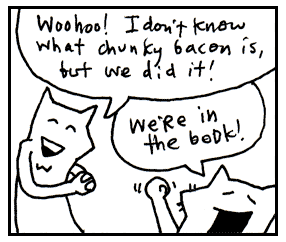
\includegraphics[width=0.25\textwidth]{image/why/foxes-4f.png}
  \caption{哇呜! Chunky bacon的点子终于用上了. }
\end{figure}

\subsection*{Blocks}
被一对\textbf{花括号}包裹起来的代码就是一个block(代码块). 

\begin{quotation}
  \begin{minted}{ruby}
    2.times {
      print "Yes, I've used chunky bacon in my examples, but never again!"
    }
  \end{minted}
\end{quotation}

有了block, 你就可以将一串指令打包在一起, 
然后它们就能够在你的程序里面相互传递. 
\footnote{原文是: With blocks, you can group a set of instructions together so that they can be passed around your program. 可以从中看出运行过程的抽象, 将指令(或者说是函数? )当作了数据来看. }
这一对花括号就像是一对蟹钳, 紧紧地将里面的代码钳住. 
所以无论何时你看见了这一对花括号, 请记得把里面的代码当作是一个整体. 

这就有点像是那些在商场里面销售那些印有Hello Kitty的文具大礼盒. 
透过华丽的透明包装纸可以看见里面塞满了成套的小铅笔和小纸片, 
这些漂亮的小玩意儿在光照下闪闪发光, 让你忍不住想要伸手把它们拿起来, 
然后在纸上试试. 
\footnote{原文: It's like one of those little Hello Kitty boxes they sell at the mall that's stuffed with tiny pencils and microscopic paper, all crammed into a glittery transparent case that can be concealed in your palm for covert stationery operations. 我应该改变了很多的原文的意思, 但是这个长难句实在有点难以分析. (笑) 所以我选择意译.}
不过我们的block却不需要那么多华丽的包装罢了. 

你也可以把那对花括号换成\textbf{do}和\textbf{end}. 
这样在你的代码比较长的时候(比如多于一行)就会看起来漂亮一些. 

\begin{quotation}
  \begin{minted}{ruby}
    loop do
      print "Much better."
      print "Ah.  More space!"
      print "My back was killin' me in those crab pincers."
    end
  \end{minted}
\end{quotation}

\subsection*{Block arguments}
Block arguments(代码块参数)的形式是\textbf{管道符(pipe characters)}
\footnote{呃, 其实也可以叫得土一点, 就叫竖杠就行了. 但是这个"竖杠"在命令行操作里面干的事情确实和管道很像, 就是将参数(输出)传送到另外的一个程序里面, 就像一个管道一样. 而在 Ruby 里面, 它干的事情也和参数传递有关. 所以翻译成管道符我觉得比较好. }
包裹着的一组用\textbf{逗号}分隔的variable. 

\begin{quotation}
  \mintinline{ruby}{|x|}, \mintinline{ruby}{|x, y|}以及\mintinline{ruby}{|up, down, all_round|}就是一些例子
\end{quotation}

Block arguments 一般用在block的开头: 

\begin{quotation}
  \begin{minted}{ruby}
    { |x, y| x + y}
  \end{minted}
\end{quotation}

在上面的例子里面, \mintinline{ruby}{|x, y|}就是输入的参数(arguments).
我们小小的一片代码就跟在参数的后面: \mintinline{ruby}{x + y}
将两个参数加在一起. 

我比较倾向于将管道符看作是一个管道(tunnel)的象征. 
它们看起来就像是滑滑梯一样, variables从上面滑下来. 
(\mintinline{ruby}{x}展开双臂, 想像雄鹰展翅一般冲了下来, 而\mintinline{ruby}{y}则优雅地交叉着腿滑了下来. )
这个滑梯就像是一个连接着周围世界和block的一条神奇通道. 
\footnote{奇蛋物语里面的游乐场的滑滑梯给了我翻译的灵感. 原文大概应该也是这个意思: I like to think of the pipe characters as representing a tunnel. They give the appearance of a chute that the variables are sliding down. (An x goes down spread eagle, while the y neatly crosses her legs.) This chute acts as a passageway between blocks and the world around them.}

Variables就是通过这个滑滑梯(或者说是管道)进入到block里面的. 

\begin{figure}
  \centering
  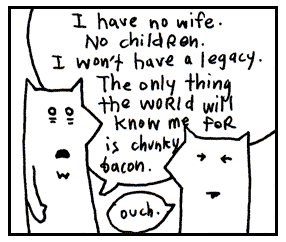
\includegraphics[width=0.25\textwidth]{image/why/foxes-4g.png}
  \caption{然后是悲惨的现实}
\end{figure}

\subsection*{Ranges}
两个用\textbf{括号}包围, 并且用\textbf{省略号}
(虽然大部分情况下, 这个省略号是用两个点来表示的)
分隔的variable就是一个range的主要形式. 

\begin{quotation}
  \begin{itemize}
    \item \mintinline{ruby}{(1..3)} 就是一个range, 代表着从$1$到$3$的数字. 
    \item \mintinline{ruby}{('a'..'z')} 也是一个range, 代表着小写的从a到z的一组字母. 
  \end{itemize}
\end{quotation}

你不妨将它想象成一个被压缩在一起拿着的手风琴. 
(但是你当然也可以特立独行, 故意拖着不收起来的手风琴在路上走, 
绝对会是街上的一道风景. 但是人有时候还是需要一些自我反省的, 
所以我建议你还是小心地把手风琴收起来. )那组括号就是手风琴的两个小把手.
然后那些点号就是合上手风琴的链子(chain), 让那些褶皱紧紧的合着. 

通常, 我们只用两个点号. 但是如果一个range里面用了三个点号, 
这就表明最后的那个值将会被剔除. 

\begin{quotation}
  \begin{itemize}
    \item \mintinline{ruby}{(1...5)} 代表$0$到$4$的数字. 
  \end{itemize}
\end{quotation}

所以当你看到三个点号的时候, 想象一下一个微微打开的手风琴. 
恰好让一个小小的音符逃了出来, 对于这最后一个音符, 
我们不妨就让它随风而去吧. 
\footnote{原文更有诗意: When you see that third dot, imagine opening the accordion slightly. Just enough to let one note from its chamber. The note is that end value. We'll let the sky eat it. 俺没文化, 翻译得不够好. }

\subsection*{Arrays}
一列用\textbf{逗号}分隔并且被\textbf{方括号}包围的东西就是array(数组).

\begin{quotation}
  \begin{itemize}
    \item \mintinline{ruby}{[1, 2, 3]} 就是一个装着数字的array. 
    \item \mintinline{ruby}{['coat', 'mittens', 'snowboard']} 是一个装着字符串的range. 
  \end{itemize}
\end{quotation}

你不妨想象这样的一个场景, array就像是一只毛毛虫被钉在了你的代码里面. 
那两个方括号就像是阻止毛毛虫移动的钉子, 这样你就可以知道哪里是它的头, 
哪里是它的尾. 然后逗号就像是它的小脚, 在它身体的节与节之间摇摆. 

从前有一只毛毛虫长着用逗号做的小腿, 
于是他不得不在每一个字面上的间隔上做一次停顿. 
为此其他的毛毛虫都非常地尊重他, 所以他变得非常有威严. 
噢, 还有一个喜欢给那些不幸的小虫子送新鲜树叶的臭名昭著的慈善家. 
\footnote{这段不是很好翻译, 在翻译上请教了别人, 原文: Once there was a caterpillar who had commas for legs. Which meant he had to allow a literary pause after each step. The other caterpillars really respected him for it and he came to have quite a commanding presence. Oh, and talk about a philanthropist! He was notorious for giving fresh leaves to those less-fortunate.\\在这里我给出一个比较随便的讲法: array就是一组有顺序排列的东西. 就像是毛毛虫的身体一样, 一节一节的, 每一节里面都放着一个东西, 毛毛虫有头有尾, 所以类似的, 这些一节一节的都是有顺序的. }

是的, 一个array就是一堆东西的集合, 
但是arrary同时也会将自己里面的东西按照一定的顺序进行储存. 

\subsection*{Hash}
一个hash(哈希)就像是一本被\textbf{花括号(curly braces)}
包在一起的字典. 没错, 就像是字典一样 -- 字典将单词和他们的定义配对 --
Ruby 里面用一个\textbf{箭头(=>)}来将两个东西配对起来. 这个箭头, 
正如你所见, 就是一个等号和一个大于号组成的. 

\begin{quotation}
  \mintinline{ruby}{{'a' => 'aardvark', 'b' => 'badger'}} 就是一个例子. 
\end{quotation}

我们这个时候不妨将这对花括号想象成一本书的封皮(book symbols), 
里面的逗号就像是每一页的边角, 见过书中间(书脊)折起来的部分吗? 
他们代表着打开和折叠这本字典的历史. 

翻开我们想象的字典, 将它平摊在桌面上, 每一页都是一个定义, 
然后我们的逗号代表着页脚, 然后我们就可以翻到下一页. 在每一页上, 
\footnote{这里不妨这样想, 左边一面是单词, 中间就是我们的"箭头", 右边一面是定义, 然后书的边角是逗号}

\section*{译后记}
怎么说呢, 感觉why先生的语言实在是妙, 在书中有各种各样的双关, 
明喻和暗喻等等, 翻译起来的难度比较大. 
然后发现网上已经有人给了一个\href{http://codecly259.github.io/poignant-guide-cn/book/chapter-3.html}{翻译}了, 
虽然没有完全翻译, 但是这个版本的翻译应该是比较标准的. 

既然有了比较标准的翻译了, 所以我就决定放飞自我了, 
做一个比较随意的翻译了. 但是在编程部分我一定会认真翻译, 
并且尽可能地去做注记的. 帮助你能够看懂. 虽然原书就已经非常容易理解了.

假如你觉得不太好的话, 建议还是去看原书吧. 